\documentclass[tikz,border=3mm]{standalone}
\usepackage{pgfplots}
\pgfplotsset{compat=1.17}
\begin{document}
	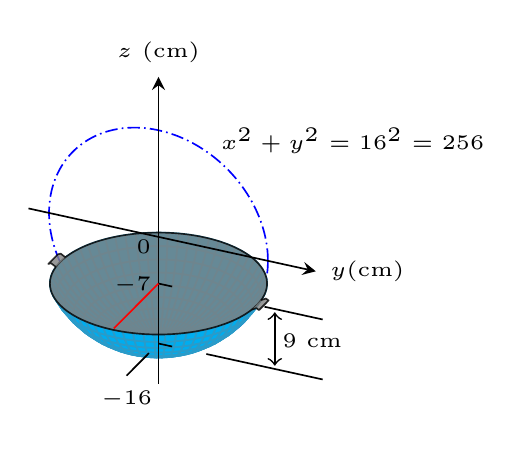
\begin{tikzpicture}[scale=1.5,join=round]
		\begin{axis} [hide axis,axis equal, view={115}{28},xmax=24, ymax=24, zmax=24]
			\addplot3[domain=0:2*pi, densely dash dot, samples=100, samples y=0, no marks, smooth, blue]({0},{16*cos(deg(x))},{16*sin(deg(x))});
			\addplot3[surf, colormap=
			{cyangray}{color=(cyan) color=(cyan)},domain=29*pi/45:pi,y domain=0:2*pi,samples = 11, samples y=64,z buffer = sort,] ({16*sin(deg(x))*cos(deg(y))},{16*sin(deg(x))*sin(deg(y))},{16*cos(deg(x))});
			\addplot3[fill=gray,opacity=.8,domain=0:2*pi, samples=100, samples y=0, no marks, smooth]({sqrt(207)*cos(deg(x))},{sqrt(207)*sin(deg(x))},{-7});
			\draw[-stealth] (0,-19,0)--(0,23,0)node[right]{\tiny $y$(cm)};
			\draw[-stealth] (0,0,-22)--(0,0,24)node[above]{\tiny $z$ (cm)};
			\draw (0,0,-7)--(0,2,-7) (0,15.5,-7)--(0,24,-7) (0,0,-16) --(0,2,-16) (0,7,-16)--(0,24,-16) (3,0,-16)--(10,0,-16);
			\draw[<->] (0,17,-15.5)--(0,17,-7.5);
			\draw[red] (0,0,-7)--(14,0,-7);
			\draw (0,7,16)node[right]{\tiny $x^2+y^2=16^2=256$} (0,16,-12)node[right]{\tiny 9 cm} (0,1,2)node[below left]{\tiny $0$} (0,1,-7)node[left]{\tiny $-7$} (10,0,-16)node[below]{\tiny $-16$};
			\draw[fill=gray,opacity=.8] (-1.5,14.3,-7)--(-1.5,15,-6.6)--(-1.5,15.4,-6.8)--(1.5,15.4,-6.8)--(1.5,15,-6.6)--(1.5,14.3,-7)
			(-1.5,-14.3,-7)--(-1.5,-15,-6.6)--(-1.5,-15.4,-6.8)--(1.5,-15.4,-6.8)--(1.5,-15,-6.6)--(1.5,-14.3,-7);
		\end{axis}
	\end{tikzpicture}
\end{document}